%%%%%%%%%%%%%%%%%%%%%%%%%%%%%%%%%%%%%%%%%%%%%%%%%%%%%%%%%%%%%%%%%%%%%%%%

%%% LaTeX Template for AAMAS-2027 (based on sigconf.tex)
%%% Prepared by the AAMAS-2027 Publication Chairs based on the version from AAMAS-2026.

%%%%%%%%%%%%%%%%%%%%%%%%%%%%%%%%%%%%%%%%%%%%%%%%%%%%%%%%%%%%%%%%%%%%%%%%

%%% Start your document with the \documentclass command.


%%% == IMPORTANT ==
%%% Use the first variant below to anonymize your submission (no author information shown).
%%% Use the second variant below for the final paper (including author information).
%%% For further information on anonymity and double-blind reviewing,
%%% please consult the call for paper information
%%% https://warwick.ac.uk/fac/sci/dcs/aamas2027/calls/

%%%% For anonymized submission, use this
\documentclass[sigconf,anonymous]{aamas}

%%%% For camera-ready, use this
%\documentclass[sigconf]{aamas}


%%% Load required packages here (note that many are included already).

\usepackage{tikz}
\usetikzlibrary{arrows.meta}
\usepackage{balance} % for balancing columns on the final page

%%%%%%%%%%%%%%%%%%%%%%%%%%%%%%%%%%%%%%%%%%%%%%%%%%%%%%%%%%%%%%%%%%%%%%%%

%%% AAMAS-2027 copyright block (do not change!)

\makeatletter
\gdef\@copyrightpermission{
  \begin{minipage}{0.2\columnwidth}
   \href{https://creativecommons.org/licenses/by/4.0/}{
\includegraphics[width=0.90\textwidth]{by}}
  \end{minipage}\hfill
  \begin{minipage}{0.8\columnwidth}
   \href{https://creativecommons.org/licenses/by/4.0/}{This work is licensed under a Creative Commons Attribution International 4.0 License.}
  \end{minipage}
  \vspace{5pt}
}
\makeatother

\setcopyright{ifaamas}
\acmConference[AAMAS 2027]{Proc.\@ of the 26th International Conference
on Autonomous Agents and Multiagent Systems (AAMAS 2027)}{3--7 May 2027}{Hanoi, Vietnam}{M.~Baldoni, F.~Fang, W.~Yeoh, N.~Yorke-Smith (eds.)}
\copyrightyear{2027}
\acmYear{2027}
\acmDOI{}
%\acmPrice{}
\acmISBN{}

%%%%%%%%%%%%%%%%%%%%%%%%%%%%%%%%%%%%%%%%%%%%%%%%%%%%%%%%%%%%%%%%%%%%%%%%

%%% == IMPORTANT ==
%%% Use this command to specify your OpenReview submission number.
%%% In anonymous mode, it will be printed on the first page.

\acmSubmissionID{Layout preview only}

%%% Use this command to specify the track you want to submit your paper to.

\submissionType{Research Paper Track}
%\submissionType{AAAI Track}
%\submissionType{Demonstration Track}
%\submissionType{Blue Sky Ideas Track}
%\submissionType{JAAMAS Track}
%\submissionType{Doctoral Consortium}

%%% Use this command to specify the title of your paper.


\title{Workflow figure layout preview}
\begin{abstract}
This technical preview checks a workflow diagram in the unchanged AAMAS 2027
class. It contains no experimental results and is not a conference submission.
\end{abstract}
\keywords{Workflow layout, figure preflight}
\begin{document}
\maketitle
\section{Layout check}
The next page uses a full-width figure at native size, without scaling the text.
The scientific paper will identify all task counts, model settings and outcome
rules in its methods. This preview does not replace the final scientific or
visual review of that paper.
\begin{figure*}[t]
\centering
% Reusable full-width figure; no experimental outcomes or submission claim.
% Model-call boxes are solid. Host-execution boxes are dashed.
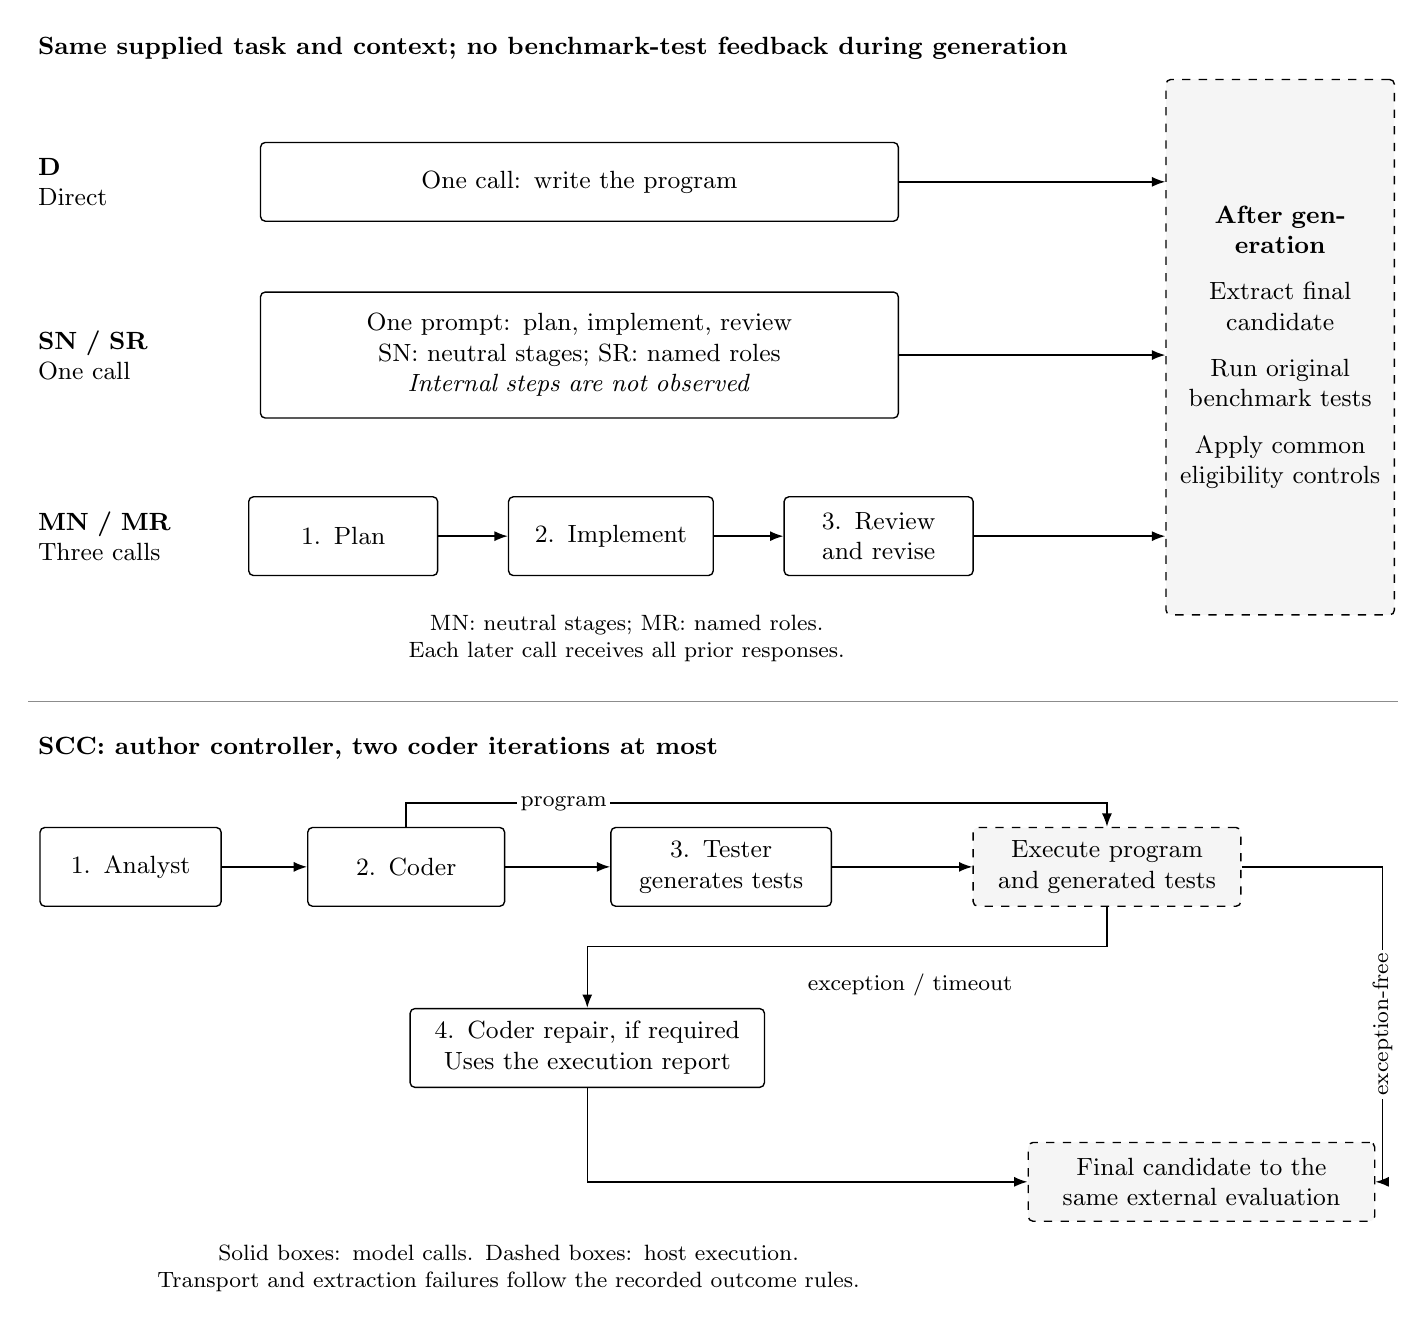
\begin{tikzpicture}[x=1mm,y=1mm,
 call/.style={draw=black,line width=.5pt,rounded corners=.6mm,align=center,
              font=\small,inner sep=1.5mm,minimum height=10mm},
 host/.style={call,dashed,fill=black!4},
 flow/.style={-{Latex[length=1.7mm]},line width=.55pt},
 lab/.style={font=\small,align=left,anchor=west},
 note/.style={font=\footnotesize,align=center}]
\node[lab,font=\small\bfseries] at (0,0) {Same supplied task and context; no benchmark-test feedback during generation};

\node[lab,text width=24mm] at (0,-17) {\textbf{D}\\Direct};
\node[call,text width=78mm] (direct) at (70,-17) {One call: write the program};
\node[host,text width=26mm,minimum height=68mm] (final) at (159,-38)
 {\textbf{After generation}\\[2mm]Extract final\\candidate\\[2mm]Run original benchmark tests\\[2mm]Apply common eligibility controls};
\draw[flow] (direct.east) -- (final.west |- direct.east);

\node[lab,text width=25mm] at (0,-39) {\textbf{SN / SR}\\One call};
\node[call,text width=78mm,minimum height=16mm] (single) at (70,-39)
 {One prompt: plan, implement, review\\SN: neutral stages; SR: named roles\\\emph{Internal steps are not observed}};
\draw[flow] (single.east) -- (final.west |- single.east);

\node[lab,text width=25mm] at (0,-62) {\textbf{MN / MR}\\Three calls};
\node[call,text width=21mm] (plan) at (40,-62) {1. Plan};
\node[call,text width=23mm] (code) at (74,-62) {2. Implement};
\node[call,text width=21mm] (revise) at (108,-62) {3. Review\\and revise};
\draw[flow] (plan) -- (code);
\draw[flow] (code) -- (revise);
\draw[flow] (revise.east) -- (final.west |- revise.east);
\node[note,text width=106mm] at (76,-75) {MN: neutral stages; MR: named roles. Each later call receives all prior responses.};

\draw[black!45,line width=.4pt] (0,-83) -- (174,-83);
\node[lab,font=\small\bfseries] at (0,-89) {SCC: author controller, two coder iterations at most};
\node[call,text width=20mm] (analyst) at (13,-104) {1. Analyst};
\node[call,text width=22mm] (coder) at (48,-104) {2. Coder};
\node[call,text width=25mm] (tester) at (88,-104) {3. Tester\\generates tests};
\node[host,text width=31mm] (execute) at (137,-104) {Execute program\\and generated tests};
\draw[flow] (analyst) -- (coder);
\draw[flow] (coder) -- (tester);
\draw[flow] (tester) -- (execute);
\draw[flow] (coder.north) -- ++(0,3) -| (execute.north);
\node[note,fill=white,inner sep=.4mm] at (68,-96) {program};
\node[call,text width=42mm] (repair) at (71,-127) {4. Coder repair, if required\\Uses the execution report};
\node[host,text width=41mm] (sccfinal) at (149,-144) {Final candidate to the\ same external evaluation};
\draw[flow] (execute.south) -- ++(0,-5) -| (repair.north);
\node[note,fill=white,inner sep=.4mm] at (112,-119) {exception / timeout};
\draw[flow] (execute.east) -- (172,-104) -- (172,-144) -- (sccfinal.east);
\node[note,rotate=90,fill=white,inner sep=.4mm] at (172,-124) {exception-free};
\draw[flow] (repair.south) -- (71,-144) -- (sccfinal.west);
\node[note,text width=115mm] at (61,-155)
 {Solid boxes: model calls. Dashed boxes: host execution.\\Transport and extraction failures follow the recorded outcome rules.};
\end{tikzpicture}

\caption{Generation workflows and their evaluation boundary. D, SN, SR, MN and
MR are the five factorial conditions. In a separate contemporaneous study, SCC
is compared with fresh SN and SR using the same model. SCC's generated tests are
not the hidden benchmark tests. The diagram shows ordinary completion paths;
transport aborts and author-code extraction fallbacks are handled separately.
An exception-free internal run does not establish benchmark correctness.
The configured SCC controller does not retest a repaired program internally.}
\Description{Three factorial configurations produce a single final program:
a direct request; one request with three prescribed operations; and three
sequential calls forwarding all previous responses. Each is evaluated after
generation using the benchmark tests and common controls. The SCC workflow has
analyst, coder and tester calls followed by isolated execution of the generated
tests. Execution without an exception stops the session; an exception or timeout
can lead to one coder repair. Both paths lead to the same external evaluation.
Hidden benchmark tests are never returned to the model.}
\end{figure*}
\clearpage
\end{document}
